%%%%%%%%%%%%%%%%%%%%%%%%%%%%%%%%%%%%%%%%%%%%%%%%%%%%%%%%%%%%%%%%%%%
%                                                                 %
%                            CHAPTER TWO                          %
%                                                                 %
%%%%%%%%%%%%%%%%%%%%%%%%%%%%%%%%%%%%%%%%%%%%%%%%%%%%%%%%%%%%%%%%%%%

\chapter{ARRAY-BASED MESH REPRESENTATIONS}
\let\thefootnote\relax\footnotetext{
Portions of this chapter submitted as:
D. Ibanez and M. Shephard,
``Modifiable Array Data Structures for Mesh Topology,"
in \textit{SIAM J. Scientific Comput.},
under review.
}
\label{chap:struct}

This Chapter presents two data structures, each used to represent
the portion of the mesh (a.k.a. \emph{mesh part}) stored in one
shared memory space.
Each of these structures are augmented with information connecting multiple
mesh parts across distributed memory spaces as described in
Chapter \ref{chap:parallel}, the result of which is a pair of fully parallel
mesh data structures.

\section{Goals}
\label{sec:struct_goals}

An unstructured mesh simulation code relies heavily on
multiple core capabilities to deal with the mesh,
and the range of features available at this level constrain
the capabilities of the simulation as a whole.
As such, the long-term goal towards which this thesis
contributes is the development of a mesh data structure
with the following capabilities:

\begin{enumerate}
\item The flexibility to adapt to evolving meshes
\item The ability to represent any of the conforming meshes typically
used by Finite Element (FE) and Finite Volume (FV) methods
\item Low memory use
\item High locality of storage
\item Highly scalable implementation for distributed memory computers
\item The ability to parallelize work inside heterogeneous
supercomputer nodes
\end{enumerate}

The first goal is the most consequential.
If adaptivity is implemented as a series of requests to
add and remove mesh entities, then a much more complex structure is required
(see Section \ref{sec:def_adapt} for further discussion).
Such a structure is described in Section \ref{sec:sisc}.
However, this approach tends to conflict with our sixth goal regarding
on-node parallelism.
Therefore we also present an alternative
approach in which the additions and removals required for adaptivity
are accumulated into batches to be applied all at once
(see Section \ref{sec:indset}), which allows us to use a less complex structure
as presented in Section \ref{sec:omega_h-struct} while adhering to the
principles of on-node programming established in Sections
\ref{sec:openmp} and \ref{sec:cuda}.

\section{Related Work}

There are several other implementations of mesh data structures
which offer various subsets of the features described herein:

First, there are dynamic structures which support mesh adaptation.
FMDB is an object-oriented structure that
stores full one-level representations \cite{seol2006efficient}.
It is capable of constant-time local
mesh modifications and supporting adaptation code.
Similar to FMDB is the mesh databased used by Comp\`{e}re and Remacle
in the MAdLib adaptation package \cite{compere2010mesh}.
Celes, Paulino, and Espinha also implement a structure capable of
adaptation \cite{celes2005compact}.
Another example of an adaptive structure
is the GRUMMP system developed by Ollivier-Gooch
and available at \texttt{http://tetra.mech.ubc.ca/GRUMMP}.

Second, there are array-based structures designed for
efficient access of unchanging meshes.
STK is an array-based mesh structure being developed at
Sandia National Laboratory \cite{edwards2010sierra}.
MOAB is another array-based structure developed primarily
at Argonne National Laboratory \cite{tautges_moab:_2004},
and working with MOAB an Adjacent Half-Facet structure
was implemented which can perform some modifications \cite{dyedov2014ahf}.

\section{Choices in Representation}

There are key choices in terms of which entities
and adjacencies to store which apply equally well
to both of the structures presented in this Chapter.

\subsection{Choosing Entities to Store}

Unstructured mesh applications must represent
the portions of the mesh topology graph
needed to support the operations carried out on the mesh.
A representation which explicitly stores
every entity is said to be a {\it full}
representation.
Any schemes which allow some entities to be represented
implicitly (i.e. their presence does not consume memory)
are {\it reduced} representations.

As we began to discuss in Section \ref{sec:def_adapt},
there are multiple factors in the decision of which entities to store:
\begin{enumerate}
\item For boundary condition application, it is necessary to
be able to infer the classification of mesh faces.
\item For mesh adaptivity, it is necessary to be able to
infer the classification of any mesh entity, whether stored or not.
\item In mesh adaptation, it is often useful to store values
on the edges and vertices (for example, booleans indicating they
are candidates for modification).
\item If the basis functions used for PDE discretization have
degrees of freedom on edges or faces, those edges and faces
must be stored.
\end{enumerate}

There are also many consequences of storing only a subset of entities that
must be considered:
\begin{enumerate}
\item If some entities of a given dimension are not stored, then
downward adjacencies from a higher dimension to the partially-stored dimension
would need to be more complex.
\begin{enumerate}
\item Given a single high-dimensional entity, the ordering of its
adjacent bounding entities is crucial.
If some of them are not stored, the remaining adjacency relationships
would need to be annotated with ordering information such that the correct
ordering can still be reconstructed.
\item Depending on the implementation, downward adjacencies would either
not have constant degree of have ``null" values where non-stored entities
are adjacent.
Both would complicate all code that queries and manages
downward adjacencies.
\end{enumerate}
\item How to query information (such as classification) about a non-stored
entity is unclear. FMDB took the approach of temporarily creating
and storing those entities when queries were made \cite{seol2005fmdb}.
Celes, Paulino, and Espinha use a similar solution in their reduced
representation \cite{celes2005compact}.
This workaround is incompatible with portable execution, as GPUs
would not allow creating entities individually in this manner.
\end{enumerate}
Beall and Shephard indicate other complexities involved
with handling reduced representations \cite{beall1997general}.

Given that adaptation would require us to store edges and boundary
faces, we are left only considering whether to introduce great
complexity in exchange for not storing interior faces.
In this work we choose instead to store all entities.

\subsection{Choosing Adjacencies to Store}

Once the set of explicit entities is chosen, one has
options about which adjacencies to store.
Recall from Section \ref{sec:def_adj} that downward and upward
adjacencies are transitive, so there are many
subsets of the adjacencies from which the others
can be reconstructed.
For any given representation, the computation of $M^d_i\{M^q\}$
can either be done efficiently using stored information
or using an exhaustive search if less information is available.
If one can compute $M^d_i\{M^q\}$ for a single
given entity $M^d_i$ in constant time,
we say that the stored information is {\it complete} \cite{seol2006efficient}.
Recall from Section \ref{sec:def_fem} that upward adjacencies
are bound by a constant, so they are computable in
constant-time if enough information is stored.

A comparison of representations based on the choice
of dimensions and adjacencies between
dimensions to represent
was published by Garimella \cite{garimella2002mesh}.
The choices we made in our structures are described separately
for each data structure,
in Sections \ref{sec:mds_adj} and \ref{sec:omega_h-struct}.

\section{MDS Data Structure}
\label{sec:sisc}

The MDS structure is built around the following key characteristics:

\begin{enumerate}
\item The representation centers around graph theoretic interpretations
of topological adjacency.
\item The mesh can remain topologically consistent with and associated with
geometric model entities.
\item The common element types of FE/FV methods can coexist in one structure.
\item Additional data can be associated with entities to implement
high order basis functions, including for geometric approximation.
\item A mesh can be modified by adding and removing single entities in constant time.
\item The entire mesh is stored in a few contiguous dynamic arrays.
\end{enumerate}

One key contribution of this thesis is to show that the latter two properties,
array storage and rapid single-entity modification, are not mutually exclusive
and can be combined in a viable way.

\subsection{Adjacencies stored in MDS}
\label{sec:mds_adj}

MDS is based on the full {\it one-level} representation,
in which we store the upward
and downward adjacencies between each consecutive
pair of dimensions \cite{beall1997general}.
In particular, it stores
region-face, face-edge, and edge-vertex adjacencies
(both upward and downward).
Despite this focus on the one-level adjacencies, the general MDS
structure can be used to store any subset of
adjacency relations.

\begin{figure}
\begin{center}
\includegraphics[width=0.53\textwidth]{full_rep.png}
\caption{A geometric representation of one-level
relations among a subset of the entities that bound a tetrahedron.}
\label{fig:mds_topo}
\end{center}
\end{figure}

\begin{figure}
\begin{center}
\includegraphics[width=0.8\textwidth]{adjs_mds.png}
\caption{Single-entity adjacency derivations in MDS.}
\label{fig:adjs_mds}
\end{center}
\end{figure}

Figure \ref{fig:mds_topo} illustrates geometrically the relationships
stored in a full one-level representation.
Each arrow representing an adjacency relation (a.k.a. entity use)
is bi-directional to indicate that we store both the
downward (high to low dimension) and upward (low to high) relations.
Note that vertices are related only to edges,
regions are related only to faces, etc.

MDS stores these one-level adjacencies directly
and updates them as needed during entity addition and removals,
so we can call them the ``permanent" adjacencies.
In order to fulfil requests for any adjacency information regarding a single
mesh entity at runtime,
MDS it carries out derivations based on the permanent adjacency information
as shown in Figure \ref{fig:adjs_mds}.

Downward adjacencies not directly stored are derived
locally by intersecting existing adjacencies.
For example, the vertices of a triangle may be found
by querying its edges and then the vertices of those
edges, and ordering is preserved by finding a vertex
that is adjacent to two particular edges.
Such intersection logic moves down one dimension, and
can be repeated if needed.

Conversely, upward adjacencies are found by successive
unions of existing adjacencies.
Given a vertex, one can retrieve adjacent edges, then
for each edge retrieve adjacent faces, then take the
union of these sets of faces, giving the set of unique
faces adjacent to the edge.

These derivations are based on the algorithms described
in detail in \cite{seol2005fmdb}.

\subsection{Object-Oriented Storage}
\label{sec:sisc_oo}

We begin by describing how our structure would look
if we stored it in an object-oriented manner.
In object-oriented programming, data is organized
into {\it objects} of a few {\it types}.
All objects of the same type have the same {\it attributes},
and for each object and associated attribute a {\it value} must be stored.
In the present case, the objects are mesh topological entities
and the attributes are pointers encoding adjacency relations.

The goal is to organize all data into objects whose
sizes are known at compile time based on their type.
The first step to doing this is to create separate object types
based on topological type.
Objects of the same type are all topologically similar to some polytope,
for example a triangle or a pyramid.
This ensures that their downward adjacency degrees are all the same,
which makes downward adjacency storage fairly straightforward.
For example, a tetrahedron in a full representation would store
four pointers to its bounding faces.

\begin{figure}
\begin{center}
\includegraphics[width=0.9\textwidth]{oo.png}
\caption{(left) the example mesh: a reduced representation of two
triangles sharing one edge and two vertices.
(middle) the linked-list storage of upward adjacency information
for vertices to triangles.
(right) a key describing the meaning of symbols in the middle figure}
\label{fig:oo}
\end{center}
\end{figure}

The second step is to use a linked-list technique \cite{karamete2016novel}
to distribute upward-adjacency storage amongst the entities
of higher dimension, alleviating the need for variable-length
storage in lower-dimensional objects.
If an object stores $m$ downward pointers, then it also stores
$m$ singly-linked list nodes.
A singly-linked list node simply contains a pointer to the next
node, which can also be null.
Every low-dimensional object then stores a single ``head" node
which begins their upward linked list.
If a high-dimensional object ($h$) points to a low-dimensional object ($l$)
from its $j$th downward pointer, then its $j$th list node must be
part of object $l$'s linked list.
Figure \ref{fig:oo} illustrates this portion of the data structure
for a reduced mesh of two triangles.
Notice how, for a shared vertex, one begins at the vertex's head node,
reaches a node that is stored for triangle 0, then continues
to a node stored for triangle 1, which contains a null pointer.
This is fundamentally how upward adjacency is queried for a vertex.
A singly-linked list can be used as opposed to doubly-linked one
because per Section \ref{sec:def_mesh}
the number of nodes in this list has a constant upper bound.
This means we can afford the $O(m)$ runtime cost of removing a node from this
list when a high-dimensional entity is removed
($m$ being the number of upward adjacent entities),
in exchange for halving the memory use.

\subsection{Structure of Arrays}
\label{sec:sisc_soa}

Next we describe how we convert the object-oriented structure
into an array-based one.
Instead of storing all data for a single object contiguously,
i.e. organizing by object first and then by attribute,
we organize data first by attribute and then by object.
We store all data for a single attribute in a contiguous
array, hence this scheme can be called a {\it structure of arrays}
\cite{sung2012dl}.
In our case, examples of attribute arrays would be
the ``first up" nodes for all entities of dimension $d$
and likewise the ``next up" nodes for all entities of dimension $(d+1)$.
For a static mesh we would be done, but this structure needs
to support efficient addition and removal of objects.
We therefore need to manage the arrays which store attributes
for all objects a single type, to account for addition and removal
of objects of that type.

When users request the addition of a new entity, we are allowed
to store it anywhere in the structure.
In this case adding objects in constant time has a well-known
solution called geometric growth \cite{cormen2001table}.
At any time we have some amount of array storage capacity $c(t)$
which is filled entry at a time.
When that storage is full, we reallocate it to a new capacity $c(t+1)$,
such that the integer function $c(t)$ approximates the real function
$f(t) = \alpha^t$, where $1< \alpha\leq 2$.
Although reallocation has a runtime cost of $O(c(t))$, the geometric
growth amortizes this cost such that adding objects
is constant-time on average \cite{cormen2001table}.
The tradeoff is that a bounded fraction of the storage is unused extra space.
In our case, we use a growth formula of $c(t+1) = (3(c(t)+1))/2$
as a heuristic compromise between memory and runtime.

Removing objects is usually the more troublesome operation for
array-based structures.
First, we have no control over which object is being removed.
This means a ``hole" will be created at some arbitrary index.
While some implementations opt to fill this hole immediately
with an existing object, we will avoid this because it requires
changing the index of a live object,
which causes great confusion to users
and leads to programming errors.
We prefer that object indices are like object pointers: constant
throughout the lifetime of the object.
This way a handle/pointer/index may be maintained by the user
and it will have clear meaning even during mesh modification.

If we cannot change indices then the holes must remain, and
we will track them using a free list, or list of available
space \cite{knuth1997list}.
In our implementation, this means creating a new variable array
along with those of the objects.
This array which we call the free list contains pointers
from each hole to the next hole,
and a single head pointer outside this list
points to the first hole.
We can use a singly-linked list efficiently by adding and
removing holes only to and from the front of this list,
both of which are constant-time operations.

In summary, to add an object, we first check whether there
are holes in the free list.
If so, the first hole is used as space for the object,
and it is removed from the free list.
Otherwise the object is added at the end,
which may trigger a geometric growth of all arrays
simultaneously.
To remove an object, we simply add the resulting hole as the first hole
in the free list.
See Figure \ref{fig:flex} for a helpful layout diagram
of modifiable object arrays.

\begin{figure}
\begin{center}
\includegraphics[width=0.8\textwidth]{flex.png}
\caption{Extra space and hole tracking create modifiable arrays}
\label{fig:flex}
\end{center}
\end{figure}

One issue with this structure is that memory use does
not decrease immediately when removing objects, and in theory we can
only shrink the arrays if the last object is removed.
This is connected to our decision to preserve identifiers,
and can be fixed by temporarily relaxing that constraint.
In a single collective step, all objects can be reordered,
given new identifiers, and all links between them updated
accordingly.
If the new identifiers are contiguous, the arrays can shrink
to minimal size.
As described in detail in Section \ref{sec:reorder},
this is implemented in PUMI as an operation that
combines hole removal with adjacency-based reordering
to improve locality.

An important benefit of this array-based structure is the
ease with which additional attributes can be added or removed
at runtime.
To add a new attribute to objects of the same type, we just
create a new array and ensure that subsequent resizing
operations apply to that array along with the others.
For example, different simulations may require different
attributes such as position, velocity, mass, and electrical charge.
These can each be allocated as a separate array,
and each can be added and removed at runtime as needed
with essentially no memory overhead.

\subsection{Lists in Arrays}
\label{sec:lia}

Since our initial structure composed of many small objects containing pointers
to one another was recast into a set of large arrays
as opposed to individually allocated objects,
pointers to objects get transformed into array indices.
As an example, consider the transformation for a singly-linked
list as shown in Figure \ref{fig:arraylist}.

All the list nodes are packed into an array, and a pointer to
a list node becomes an index into this array, starting with zero.
Since zero is a valid index, we can use -1 to denote a null pointer.
Notice also that if we have knowledge about the maximum length
of the array, we can choose an integer type that uses less bytes
than a pointer, since pointers must be able to index the entire
virtual address space.

\begin{figure}
\begin{center}
\includegraphics[width=0.6\textwidth]{arraylist.png}
\caption{(left) A linked list in object form.
(right) The same linked list packed into an array.}
\label{fig:arraylist}
\end{center}
\end{figure}

Since indices can have the same meaning for several arrays,
we can separate the variables in an object into different
arrays.

\subsection{Dynamically Modifiable Mesh Structure}
\label{sec:sisc_mstruct}

\begin{figure}
\begin{center}
\includegraphics[width=0.95\textwidth]{mixed.png}
\caption{(left) an example subset of a mixed mesh:
an edge adjacent to a triangle and a quad.
(right) the corresponding upward adjacency linkage
must traverse separate triangle and quad arrays.}
\label{fig:mixed}
\end{center}
\end{figure}

There is one more detail that needs resolving in the
case of mixed meshes.
The problem is that different polytope
groups may contain uses of the same entity.
For example, an edge may be used by a triangle and a quadrilateral.
They must be linked together, but their arrays are
separated by polytope group.
In order to be able to jump between those arrays, we must
enhance the indices being used.
Our solution is to encode information about the polytope group
into these indices, i.e. $e = (t,i)$ where $t$ is an integer
uniquely identifying a polytope group, $i$ is the index
into the arrays of that group, and $e$ is the extended index.
In particular, the encoding we choose is $e = iT + t$, where
$T$ is the total number of polytope groups and $0\leq t < T$.
This allows the extended index to remain an integer
and be decoded using simple modulo and division instructions.
Figure \ref{fig:mixed} illustrates this representation.
Starting with entry $20$ in the ``edge first up" array,
we are directed to edge use $2$ of quad $10$.
At entry $i=(10\cdot 4 + 2)$ of the ``quad next up" array,
we are further directed to edge use $0$ of triangle $4$.
At entry $i=(4\cdot 3 + 0)$, we find a null pointer and stop.

To get clear picture of all the arrays and their groupings
that are allocated for a real mesh, here is a listing
including all polytope types that a complex CFD mesh
might need when boundary layers are constructed with
a mix of wedges and pyramids:

\begin{enumerate}
\item Vertices
  \begin{enumerate}
  \item Coordinates (size $=3\times$vertex capacity)
  \item First edge (size $=$vertex capacity)
  \item Free list (size $=$vertex capacity)
  \end{enumerate}
\item Edges
  \begin{enumerate}
  \item Vertices used (size $=2\times$edge capacity)
  \item Next edge up (size $=2\times$edge capacity)
  \item First face up (size $=$edge capacity)
  \item Free list (size $=$edge capacity)
  \end{enumerate}
\item Triangles
  \begin{enumerate}
  \item Edges used (size $=3\times$triangle capacity)
  \item Next face up (size $=3\times$triangle capacity)
  \item First region up (size $=$triangle capacity)
  \item Free list (size $=$triangle capacity)
  \end{enumerate}
\item Quadrilaterals
  \begin{enumerate}
  \item Edges used (size $=4\times$quadrilateral capacity)
  \item Next face up (size $=4\times$quadrilateral capacity)
  \item First region up (size $=$quadrilateral capacity)
  \item Free list (size $=$quadrilateral capacity)
  \end{enumerate}
\item Tetrahedra
  \begin{enumerate}
  \item Faces used (size $=4\times$tetrahedra capacity)
  \item Next region up (size $=4\times$tetrahedra capacity)
  \item Free list (size $=$tetrahedra capacity)
  \end{enumerate}
\item Wedges
  \begin{enumerate}
  \item Faces used (size $=5\times$wedges capacity)
  \item Next region up (size $=5\times$wedges capacity)
  \item Free list (size $=$wedges capacity)
  \end{enumerate}
\item Pyramids
  \begin{enumerate}
  \item Faces used (size $=5\times$pyramid capacity)
  \item Next region up (size $=5\times$pyramid capacity)
  \item Free list (size $=$pyramid capacity)
  \end{enumerate}
\end{enumerate}
Where the capacities refer to the geometric growth
capacity described in Section \ref{sec:sisc_soa} based
on the current number of entities of that polytope group.

This structure provides a straightforward mechanism for associating
data with each entity of a polytope group by creating
new arrays as described in Section \ref{sec:sisc_soa}.
This is how vertex coordinates and entity-level fields
are stored.

\section{Omega\_h Data Structure}
\label{sec:omega_h-struct}

Omega\_h is designed for portable performance across
all the different hardware covered in Section \ref{sec:node_hw}.
As such it makes a few key decisions differently from MDS,
which affect much of its resulting structure and logic.
Apart from the focus on GPU compatibility, when designing
Omega\_h we often prefer to use more memory as opposed
to more compute time when such a trade-off is available.
Finally, Omega\_h is focused strictly on simplex mesh
adaptivity, unlike PUMI which aims also to represent
meshes containing prismatic boundary layers \cite{ovcharenko2013parallel}
or hexahedra \cite{seol2006efficient}.

\subsection{Static Mesh}
\label{sec:osh_static}

Recall from Section \ref{sec:cuda} that for effective
performance on GPUs data must be consolidated into
a few large arrays.
Both MDS and Omega\_h do this, and for the latter it is
a matter of strict necessity.

However, in MDS, the usage of the structure is clearly in terms
of requesting the creation or destruction of a single entity at
a time.
The clear benefit of this is ease of programming, but the drawback
is the inability to parallelize access to a single MDS data structure
(the free list, growth mechanism, and upward lists would become
points of contention).
For PUMI that is not a serious issue, because even with the use of
threads there will be at least a few hundred elements per thread
in typical PUMI use cases.
That means it is acceptable to have one MDS data structure per thread.
There are three reasons why this approach does not work on a GPU:
\begin{enumerate}
\item The GPU does not maintain persistent per-thread state from
one loop to another
\item The GPU has more parallelism, closer to a dozen or even
a single mesh element per compute core.
\end{enumerate}
For these reasons, Omega\_h takes a different approach:
its mesh data structure will efficiently represent a static
(unchanging) mesh topology, and the methods in Section \ref{sec:omega_h-adapt}
will construct a whole new mesh structure from the current
one, incorporating many changes at once to amortize the
cost of reconstruction.
This is the main design difference in Omega\_h: the mesh
structure is a static read-only topological structure.

\subsection{Adjacency Arrays}
\label{sec:adj_arr}

\begin{figure}
\begin{center}
\includegraphics[width=0.15\textwidth]{up_down_mesh.png}
\includegraphics[width=0.3\textwidth]{down.png}
\includegraphics[width=0.45\textwidth]{up.png}
\caption{(left) an example 4-vertex 2-triangle mesh
(middle) the downward adjacency array
(right) the upward adjacency array}
\label{fig:osh_up_down}
\end{center}
\end{figure}

This static array structure is similar to those
of the MOAB mesh database \cite{tautges2004moab},
and also of several solvers which implement their own structures.
We assume for simplicity that either all elements are tetrahedra
or they are all triangles (see Section \ref{sec:sisc_mstruct} for
the complexity associated with mixed meshes).
This allows us to store downward adjacencies in a single array
that can be thought of as two-dimensional
(see Figure \ref{fig:osh_up_down}(middle)).
Upward adjacencies (and all complex graphs in Omega\_h, for that matter)
are stored in the widely known compressed row format,
used for example in the METIS graph partitioner interface \cite{METIS}.
This consists of two arrays, one containing the destinations
of all graph edges, sorted by the source of the edge.
The second array contains offsets indicating where in the first
array the edges going out from a given graph node are stored.

\subsection{Alignment Information}
\label{sec:osh_align}

Alongside either of these adjacency representations, Omega\_h
also stores an array of useful alignment information.
A high-dimensional entity will use a low-dimensional entity
as part of its boundary. However, since that low-dimensional
entity is shared with other high-dimensional entities, in general
it will not be aligned according to the canonical orders
described in the high-dimensional entity's topological
template (see Section \ref{sec:topo_template}).
For example, a face between two regions cannot have its normal
point into both regions.
Therefore it will be ``flipped" with respect to the canonical
boundary face of one of these regions.

An alignment array has one 8-bit entry for each entity use, and encodes
data about how the entity being used lines up with the entity using it.
Although 8 bits is the smallest value that current computers allow one
to store, we only use 6 of these bits to store the following three things:
\begin{enumerate}
\item Downward ordering (3 bits): what is the canonical order of the
low-dimensional entity in the high-dimensional template.
\item Rotation (2 bits): how many times to rotate the low-dimensional
entity before it lines up with the canonical boundary
entity of the template.
\item Flip (1 bit): whether the low-dimensional entity also
needs to be flipped before it can line up with the canonical
boundary entity.
\end{enumerate}

This alignment information, if stored, can speed up a wide variety
of algorithms.
It is also typically non-trivial to compute, but can be easier
to construct at the same time as an adjacency is constructed.
For example, downward ordering is easy to construct as one
is constructing an upward adjacency based on a downward one.
Therefore the adjacency construction algorithms are the optimal
location to be computing and storing such information
(more on this in Section \ref{sec:adj_cache}).
Because they occupy only 8 bits per entity use while the
existing arrays occupy at least 32 bits per use, this additional
information consumes at most 25\% more memory, which is affordable.

\subsection{Adjacency Cache}
\label{sec:adj_cache}

In MDS, if a user requests an adjacency other than those
which are stored as per Figure \ref{fig:adjs_mds},
it is computed for the single entity the user specifies.
As mentioned in Section \ref{sec:mds_adj}, this computation
may involve complex set intersections or unions, and the
upward derivations in particular are typically implemented with
heavy use of memory allocation.
Per Section \ref{sec:cuda}, we cannot allow such frequent
and small allocations on GPUs.
In addition, we should avoid doing a lot of work in a single GPU kernel,
so it is preferable to have all the needed adjacency information stored in
a convenient manner prior to entering a GPU kernel.
Even in the MDS case, the user may request the same non-stored
adjacency information multiple times
in different contexts, and re-computing this can use significant
amounts of time (see Section \ref{sec:adj_perf}).

In profiling the execution of Omega\_h mesh adaptation, we find
the majority of time and memory is consumed by the
derivation and storage of mesh adjacencies.
To mitigate the runtime cost, our mesh structure acts as an adjacency cache,
which derives new adjacencies when they are requested and stores
them so they are available for later requests.
Figure \ref{fig:adjs_osh} shows the adjacencies that we start with
and how the others are derived.
The permanent adjacencies (those which are provided upon creation
of the mesh and uniquely define topology) are the one-level downward
adjacencies, i.e. the downward portion of Figure \ref{fig:adjs_mds}.

\begin{figure}
\begin{center}
\includegraphics[width=0.8\textwidth]{adjs_osh.png}
\caption{Full-mesh adjacency derivations in Omega\_h}
\label{fig:adjs_osh}
\end{center}
\end{figure}

We use two forms of adjacency inference:
\begin{enumerate}
\item Inversion: an upward adjacency is derived from is corresponding downward
adjacency. This reduces to a low-degree graph inversion problem, which we
solve by using atomic operations to associate graph edges with their
destination graph nodes.
The key algorithm behind adjacency inversion is included
in Appendix \ref{sec:invert_map}.
\item Transiting: Similar to the intersection process described in Section
\ref{sec:mds_adj} to derive downward adjacencies, we can combine the
downward adjacencies from dimension $p$ to dimension $(q+1)$ and
from $(q+1)$ to $q$ into a single adjacency from $p$ to $q$.
By using the alignment information stored in each downward adjacency,
we can avoid having to do any kind of set intersection, because we
can map the $(q+1)$-dimensional entities onto the $p$-dimensional template
and the template has all adjacency information stored {\it a priori}.
\end{enumerate}

Note that the set of permanent adjacencies in Omega\_h is not technically
complete, because adjacencies cannot be efficiently derived for
single entities at a time.
However, because Omega\_h does derivations on a full-mesh basis,
it can use the inversion algorithm to compute
all upward relations based on all downward relations in $O(n)$
time, whereas there is no $O(1)$ equivalent operation for a
single entity.
Thus Omega\_h obeys a relaxed definition of completeness that
requires $O(n)$ full-mesh derivation operations as opposed
to $O(1)$ single-entity derivation operations.

\section{Data Structure Performance}

\subsection{Adjacency Query Performance}
\label{sec:adj_perf}

To substantiate our claims that MDS supports $O(1)$ adjacency queries and
give an example of its typical query performance, we create two
uniform meshes at different resolutions, having approximately
100K and 200K elements, respectively.
We then time, for each pair of dimensions, how long it takes
to traverse all entities of the first dimension and query their
adjacent entities of the second dimension.
The time required to do this should be approximately the number
of entities of the first dimension times the constant time
required for one adjacency query.
Tables \ref{tab:mds_adj_100} and \ref{tab:mds_adj_200} list these timing
results for both meshes, and show fairly clearly that all times
grow by about 2X since the number of elements is about 2X larger
in the second mesh.
These timings were collected on a workstation with an Intel Xeon E5-2620v4 CPU.

\begin{table}
\caption{MDS adjacency timings (in milliseconds) for 100K tet mesh}
\label{tab:mds_adj_100}
\begin{center}
\begin{tabular}{l|r|}
dimension & entity count \\\hline
0 & 19468 \\
1 & 129010 \\
2 & 212846 \\
3 & 103303 \\
\end{tabular}
\begin{tabular}{|r|r|r r r r}
               &   & \multicolumn{4}{c}{to dimension} \\\hline
               &   &    0 &    1 &    2 &   3  \\\hline
               & 0 &      &  3.9 & 48.7 & 88.9 \\
               & 1 &  2.4 &      & 11.9 & 40.4 \\
from           & 2 & 16.2 &  4.2 &      &  9.0 \\
dimension      & 3 & 21.1 & 13.1 &  2.2 &      \\
\end{tabular}
\end{center}
\end{table}

\begin{table}
\caption{MDS adjacency timings (in milliseconds) for 200K tet mesh}
\label{tab:mds_adj_200}
\begin{center}
\begin{tabular}{l|r|}
dimension & entity count \\\hline
0 & 39696  \\
1 & 265267 \\
2 & 439107 \\
3 & 213535 \\
\end{tabular}
\begin{tabular}{|r|r|r r r r}
               &   & \multicolumn{4}{c}{to dimension} \\\hline
               &   &    0 &    1 &     2 &     3 \\\hline
               & 0 &      &  8.7 & 104.8 & 191.5 \\
               & 1 &  5.0 &      &  26.3 &  84.7 \\
from           & 2 & 33.4 &  8.7 &       &  20.3 \\
dimension      & 3 & 45.6 & 27.8 &   4.5 &       \\
\end{tabular}
\end{center}
\end{table}

Performing a corresponding study for Omega\_h is not quite
trivial.
Because Omega\_h uses an adjacency cache, the runtime cost
of querying a particular adjacency depends on which adjacencies
are already cached at the moment.
In the absolute best case, that adjacency is already cached and
need only be read directly from memory.
This best case scenario is illustrated in Table \ref{tab:osh_walk_100},
showing the time required to simply read and traverse cached adjacency
information from memory, for all entities of a given dimension,
using the same 100K mesh as Table \ref{tab:mds_adj_100}.
This data is presented as a lower bound for traversal cost, given
that Omega\_h has optimal structures for fast traversal and reading.
Table \ref{tab:osh_adj_100} presents the more useful incremental construction
times, i.e. the time required to construct an adjacency
(for all entities of the relevant dimension)
assuming any pre-requisite adjacencies used in the construction
have already been cached.
Values from Table \ref{tab:osh_adj_100} can be used in conjunction
with the diagram in Figure \ref{fig:adjs_osh} to determine
Omega\_h performance for a particular series of queries.

\begin{table}
\caption{Omega\_h traversal timings (in milliseconds) for 100K tet mesh}
\label{tab:osh_walk_100}
\begin{center}
\begin{tabular}{|r|r|r r r r}
               &   & \multicolumn{4}{c}{to dimension} \\\hline
               &   &    0 &    1 &    2 &   3  \\\hline
               & 0 &      &  0.2 &  0.2 &  0.2 \\
               & 1 &  1.7 &      &  1.4 &  1.4 \\
from           & 2 &  2.6 &  2.7 &      &  2.3 \\
dimension      & 3 &  1.2 &  1.2 &  1.3 &      \\
\end{tabular}
\end{center}
\end{table}

\begin{table}
\caption{Omega\_h incremental construction timings (in milliseconds) for 100K tet mesh}
\label{tab:osh_adj_100}
\begin{center}
\begin{tabular}{|r|r|r r r r}
               &   & \multicolumn{4}{c}{to dimension} \\\hline
               &   &    0 &    1 &    2 &   3  \\\hline
               & 0 &      &  7.6 & 31.1 & 16.1 \\
               & 1 &      &      & 11.1 &  9.7 \\
from           & 2 &  5.5 &      &      &  4.7 \\
dimension      & 3 &  3.2 &  9.1 &      &      \\
\end{tabular}
\end{center}
\end{table}

\section{Reordering}
\label{sec:reorder}

Array-based structures have a natural order of traversal which is to
traverse each array from start to finish.
In Omega\_h, all $d$-dimensional simplices are in one traversal order,
and in MDS there is a traversal order for each polytope topology.
Typically, mesh operations access multiple arrays but are based on
the natural ordering of a single array.
For example, a traversal based on elements may access the vertices
of each element.
Recall from Section \ref{sec:ref_comp} that the key to achieving decent
performance on most cache architectures is to access data in the order
it is stored.
Thus, we would like to establish orderings of each group (e.g. the elements)
such that accesses to other groups (e.g. the vertices) are made
in an approximately linear fashion.
Since these accesses are based on directly adjacency, what we aim to do
is order each group such that locality in the mesh (defined by graph distances)
is well correlated to locality in the array (defined by indices).
We further simplify the problem by focusing on ordering the vertices,
and define orderings for other groups based on their adjacencies to
vertices and the vertex ordering.

We interpret the mesh vertices as graph nodes and the mesh edges
as graph edges, which enables us to use the linear arrangement
measure from graph theory as our metric of locality:

\begin{equation}\label{eq:la}
\text{la}(G=(V,E)) = \sum_{(i,j)\in E} |i-j|
\end{equation}

Where $i$ and $j$ are the array indices of two graph nodes.
There is additional rationale for using this metric in the case
of finite element assembly for linear elements, which traverses
mesh vertices and accesses adjacent vertices across mesh edges.

Finding an ordering of the vertices $V$ such that Equation \ref{eq:la}
is minimized has been shown to be NP-complete for general
graphs \cite{garey1976some}.
However, our mesh-based graphs have at least two useful properties:
the degree of each vertex is bound by a small constant,
and they are equipped with an embedding of vertices into $\mathbb{R}^3$
such that Euclidean distance closely reflects graph distance.
As such, several heuristics for good linear arrangements have been developed
for meshes.
The Cuthill-McKee algorithm \cite{cuthill1969reducing},
developed to minimize the storage complexity of sparse matrices
derived from meshes, is based on
Breadth-First Search (BFS) of the graph and sorts each layer based
on the degrees of the vertices.
A similar algorithm by Zhou et al. \cite{zhou2010adjacency} based
on work by Beall and Shephard \cite{beall1997general} also
reduces to BFS for a linear mesh, and has special considerations
for the starting point of BFS.
Other (geometric) methods take advantage of the vertex coordinates,
for example by arranging vertices along the Hilbert Space-Filling Curve
(HSFC) \cite{devine2005new}.
There are also libraries implementing hierarchic methods of
graph reordering, such as METIS \cite{METIS}.
The most effective methods at minimizing the linear arrangement metric
are those which begin with one of the above methods and then apply
a form of simulated annealing in which local modifications are made
to the ordering that locally improve the metric \cite{petit2003experiments}.
However, for our purposes of cache locality it is not worth
spending a large amount of computational power to obtain a slightly
better ordering.

Table \ref{tab:la} shows the values of Equation \ref{eq:la} using
several of these methods on three different meshes:
a cube meshed with tetrahedra (1254 vertices), a fusion reactor
cross-section meshed with triangles (3695 vertices), and
a circuit solder geometry meshed with tetrahedra (2601 vertices).
The ``input" row represents the mesh's linear arrangement value
prior to reordering.
Parentheses indicate the starting node used for a search procedure,
for example BFS(0) uses the first input node as the starting point
while BFS($n-1$) uses the last input node.
For the cube, BFS(center) uses the node closest to the cube's center.
Our two main conclusions based on Table \ref{tab:la} are that
BFS and HSFC give the best (smallest) linear arrangement values,
and that the BFS result is heavily dependent on the starting point.

\begin{table}
\caption{Linear arrangement values for different meshes and heuristics}
\label{tab:la}
\begin{center}
\begin{tabular}{r|rrr}
                     &    cube &   fusion &   solder \\\hline
input                & 3163141 &  1743275 &  8688982 \\
BFS($0$)             &  678166 &   910451 &  2085725 \\
BFS($n-1$)           &  675903 &   471728 &  2098239 \\
BFS(center)          & 1106864 &      N/A &      N/A \\
HSFC                 &  597009 &   627726 &  1877633 \\
Cuthill-McKee($0$)   &  822050 &   956364 &  2161626 \\
Cuthill-McKee($n-1$) &  784566 &   501883 &  2198386 \\
METIS                & 1120368 &  1234170 &  2849735 \\
\end{tabular}
\end{center}
\end{table}

PUMI implements a BFS method with heuristics that use geometric
classification for selecting a starting node
\cite{zhou2010adjacency, beall1997general}.
One of the difficulties with the BFS method is that it is difficult
to parallelize, since layers need to be constructed sequentially.
Early versions of Omega\_h implemented a BFS method that was not
parallelized for this reason, but we did study its effects on subsequent
adaptation operations on different hardware.
Table \ref{tab:reorder-speed} shows the speedup in Omega\_h adaptation
(see Section \ref{sec:omega_h-adapt}) when a reordering is carried out
prior to each adaptation call.
Note that even though this reordering was not parallelized, there
was never a decrease in performance, and in the most extreme case
reordering made a 26-30\% difference.
This result suggests that reordering is quite beneficial and should
be incorporated into array-based adaptation workflows.

\begin{table}
\begin{center}
\caption{Locality speedups including and excluding BFS reordering time}
\label{tab:reorder-speed}
\begin{tabular}{l|r|r}
Platform           & overall & excl. reorder \\ \hline
IBM BG/Q 1 thread     &  3\% &  7\% \\
IBM BG/Q 16 threads   & 10\% & 15\% \\
IBM BG/Q 64 threads   &  5\% & 11\% \\
NVidia K40            &  2\% &  8\% \\
Intel Phi 1 thread    & 26\% & 30\% \\
Intel Phi 120 threads & 24\% & 29\% \\
Intel Phi 240 threads &  9\% & 19\% \\
Intel i7 1 thread     &  0\% &  4\% \\
Intel i7 4 threads    & 11\% & 16\% \\
Intel i7 8 threads    &  5\% & 10\% \\
\end{tabular}
\end{center}
\end{table}

Despite non-parallel BFS reordering being adequate, we would prefer
a reordering method that scales with parallelism.
The current Omega\_h code implements a Hilbert curve method (HSFC).
The Hilbert curve is a numbering of the cubes of a regular cubic grid.
Since our vertex coordinates are in a floating-point format with
52 binary digits of precision (see Section \ref{sec:repro_sum}),
we place our mesh in an implicit cubic grid that has $2^{52}$
cubes along each axis of the mesh's bounding box.
This grid never has to be represented in its entirety; there
is a constant-time algorithm for converting a coordinate in this
grid to its integer position in the Hilbert curve
\cite{skilling2004programming}.
We map each floating-point vertex coordinate to the cube it
lies in, and assign that vertex the Hilbert curve position of that
cube.
We then sort vertices by their Hilbert curve positions.
Although our resolution makes it very unlikely that two
vertices fall in the same cube, the sorting procedure would
arbitrarily order them if this did occur.
More importantly, we can use efficient sorting algorithms for
shared memory parallelism as described in Section \ref{sec:sort},
and the conversion of coordinates to Hilbert curve positions
scales linearly (see Section \ref{sec:map}), so this reordering
method is more readily parallelizable than the BFS methods.

\begin{figure}
\begin{center}
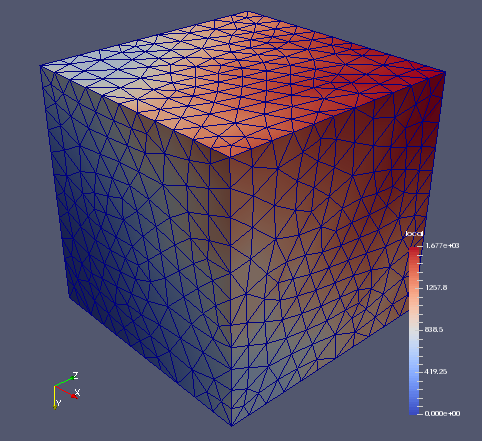
\includegraphics[width=0.4\textwidth]{bfs.png}
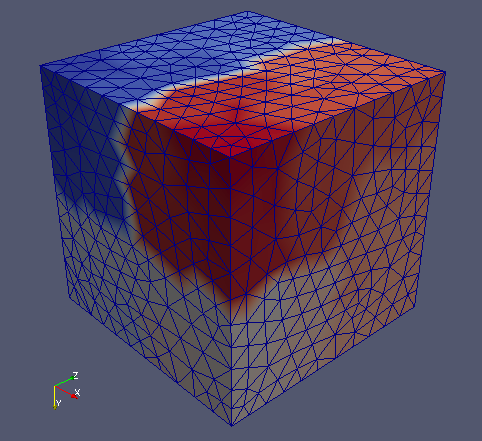
\includegraphics[width=0.4\textwidth]{hilbert.png}
\caption{Meshes colored by vertex ordering:
(left) BFS, (right) Hilbert curve}
\label{fig:reorder}
\end{center}
\end{figure}

Figure \ref{fig:reorder} shows a cube mesh with its vertices colored by
two different reordering methods: the BFS method implemented in PUMI,
and the HSFC method implemented in Omega\_h.
Blue indicates a low vertex index while red indicates a high index.
Note that while the HSFC method has a clear interface along which
indices differ highly, it should have better locality among neighbors
in the smooth areas because in the BFS method most vertices are adjacent
to vertices in the previous or subsequent layer, and those differences
are on average the size of one layer (the surface area of a cut through
the cube, measured in exposed vertices).

%%% Local Variables:
%%% mode: latex
%%% TeX-master: t
%%% End:
